\documentclass[a4paper,12pt]{article}


%calling packages
\usepackage[english]{babel}
\usepackage[utf8]{inputenc}
\usepackage{amsmath}
\usepackage{graphicx}
\usepackage[left=1in,right=1in,top=1in,bottom=1in]{geometry}
\usepackage{setspace}
\usepackage[round]{natbib}
\usepackage{epstopdf}
\usepackage{soul}
\usepackage{lmodern}
\usepackage{caption}
\usepackage{hyperref}
\usepackage{subcaption}
\usepackage{lscape}
\usepackage{rotating}
\usepackage{etoc}


\usepackage{longtable}
\usepackage{amssymb}
\usepackage{fancyhdr}
\usepackage{array}
\usepackage{lscape} % for landscape formatting of pages
\newcolumntype{P}[1]{>{\centering\arraybackslash}p{#1}}
%fonts
\usepackage{times}
%\setcounter{secnumdepth}{0}
%chanfing font of table headers
\captionsetup[figure]{labelfont=bf}
\captionsetup[table]{labelfont=bf}

%path to where figures are located
\graphicspath{ {images/} }

%for notes in table captions 
\newcommand\fnote[1]{\captionsetup{font=small}\caption*{#1}}

%changing header
\pagestyle{fancy}
\fancyhf{}
\rhead{\thepage}
\renewcommand{\headrulewidth}{0pt}
\renewcommand{\footrulewidth}{0pt}
\renewcommand*\footnoterule{}
\let\svfootnoterule\footnoterule
\renewcommand\footnoterule{\vspace{0.2in}\svfootnoterule}
\renewcommand*{\thefootnote}{\fnsymbol{footnote}}
%set spacing

\renewcommand{\sfdefault}{phv}

\doublespacing
\usepackage{titlesec}

\titleformat*{\section}{\Large\sffamily}
\titleformat*{\subsection}{\large\sffamily}
\titlespacing*\section{0pt}{24pt plus 4pt minus 2pt}{4pt plus 2pt minus 2pt}
\titlespacing*\subsection{0pt}{20pt plus 4pt minus 2pt}{4pt plus 2pt minus 2pt}


%changing title settings
\makeatletter
\renewcommand{\maketitle}{
	\begin{flushleft}
		
		\onehalfspacing
		
		\@title
		
		\lineskip .5em
		\normalfont{\normalsize{\@author}}
\end{flushleft}}
\makeatother



\newcommand{\beginsupplement}{%
	\setcounter{table}{0}
	\renewcommand{\thetable}{S.\arabic{table}}%
	\setcounter{figure}{0}
	\renewcommand{\thefigure}{S.\arabic{figure}}%
}

%title
\title{\bigskip \bigskip \sffamily \LARGE{Can Citizens Set City Policy?} \\ \Large{ Evidence From A Decentralized Welfare State}}

%author
\author{\bigskip Benjamin Carl Egerod\footnote[2]{Graduate Student, Department of Political Science, University of Copenhagen, e-mail: \texttt{benjamin.carl.egerod@ifs.ku.dk}.} \qquad Martin Vinæs Larsen\footnote[3]{Assistant Professor, Department of Political Science, Aarhus University, e-mail: \texttt{mvl@ps.au.dk}.}} 

\usepackage{xr}
\externaldocument{"citypolicy"}


\begin{document}

	
	\begin{footnotesize} \noindent \today. \end{footnotesize} %date
	
\onehalfspacing


\renewcommand{\thesubsection}{\Alph{subsection}}
\renewcommand{\thetable}{\Alph{subsection}\arabic{table}}
\renewcommand{\thefigure}{\Alph{subsection}\arabic{figure}}

\section*{Appendix: For Online Publication}

\localtableofcontents

\clearpage


\subsection{Some More Context on Danish Municipalities} 

\setcounter{table}{0}
\setcounter{figure}{0}

\label{context}
There have been two large reforms of local politics in the last 50 years in Denmark. The first was conducted in 1970 as the Danish welfare state began to expand. Here, the number of municipalities were reduced from more than 1000 to 275 \citep{ingvartsen1991kommunalreformen}. (Although it was 277 the first two years.)  The second reform was conducted in 2007 and further reduced the number of municipalities from 275 to 98. Once again, the increasing complexity of public service provision was a key argument for the reform \citep{christiansen2008utaenkelige}. Since both of these reforms were comprehensive in terms of amalgamations and changes to the relative power of national contra local government, we let them be the bookends of our analysis, examining the relationship between citizens policy views and the ideological flavor of municipal policy between the two reforms. Because of data availability we further limit our study period, so that it goes from 1978 and 2008.

In the period we study, Danish municipalities are governed by small city councils (between 9 and 29 members) that are elected at proportional elections and with a multi-party system that, to a large extent, mirrors the party system at the national level \citep{blom2013et}. Elections are fixed to take place every four years and do not usually coincide with elections at the national or EU level. Before 1981, elections always took place in the spring, but this was changed to November, so that there would be a match between calender years and election terms. To make this change there was only three and a half years between the spring 1978 and fall 1981 election. Turnout at municipal elections is high with an average of around 70 percent since 1970.  

Following each municipal election, a majority in the city council elects a mayor, and the chairmen of the various committees \citep{serritzlew2008explaining}. Mayors are the only full time professional politicians in the city councils and have a number of formal obligations \citep{kjaer2015urban}. Mayors are also responsible for the day-to-day business of the administration and chairs the important economic committee that sets taxes and the budget. The work in the city council is structured by a a number of committees. The number and size of the committees are determined by the council. Committee membership is allocated proportionally between the political parties which means that there is broad political representation in all committees. The committees can decide on matters in their area, and the administrative responsibility across areas is therefore essentially divided. 

\clearpage

\subsection{Overview of Policies Included in Our Measure} \label{policy}


\setcounter{table}{0}
\setcounter{figure}{0}

\textbf{Motivate the use of these variables and why they -- in a Danish context -- should be expected to capture fiscal conservatism.}

\begin{table}[h]
	\centering \footnotesize
	%\caption{Indicators of Fiscal Policy Conservatism}
	\label{tab:policies} 
	\begin{tabular}{p{5.5cm}P{3cm}P{4.5cm}} \hline
		\textbf{Policy}                          & \textbf{Availabiliy \newline (number of years)} & \textbf{Do Higher or Lower Values Imply Conservatism?} \\
		\hline
		&&\\ \textit{Tax policy} &&\\
		Income tax (pct.)                        & 29     &    Lower       \\
		Property tax (per mille)                      & 29    &    Lower        \\
		Commercial real estate tax (per mille) & 14    &    Lower               \\ \hline
	
		&&\\ \textit{Spending policy}  &&\\
		Spending pr. capita (DKK)                & 29    &    Lower        \\
		Spending pr. pupil in school (DKK)       & 7     &    Lower     \\ \hline
		
		&&\\\textit{Organization of public service delivery}  &&\\
 		Public Employees (pr. 1,000 citizens)	 & 9	  &	   Lower	     \\
 		Privately operated services  (pct.) &   14  &    Higher     \\
 		Purchases with a private supplier  (pct.)      & 14    &    Higher     \\ \hline
 	
 		&&\\ \textit{Co-payment for public services} &&\\   
		Average cost of day care (DKK)                  & 16    &    Higher     \\
		Price of relief stay (DKK)				 & 7	  &	   Higher	 \\
		Food delivery for the  elderly (DKK) & 7   &    Higher     \\
		Stay in nursing home (DKK)              & 7     &    Higher     \\ \hline
	
		&&\\ \textit{Extent of Public Services} &&\\ 
		Public housing (pct.)                    & 14     &    Lower               \\
		Class size in public schools	         & 14    &    Lower       \\
		\hline \hline
		\end{tabular}
\end{table} 


\begin{table}[!htbp] \centering 
	\caption{Summary Statistics on Fiscal Policy Indicators} 
	\label{tab:SumInd} 
	\begin{tabular}{@{\extracolsep{5pt}}lccccc} 
		\\[-1.8ex]\hline 
		\hline \\[-1.8ex] 
		Statistic & \multicolumn{1}{c}{N} & \multicolumn{1}{c}{Mean} & \multicolumn{1}{c}{St. Dev.} & \multicolumn{1}{c}{Min} & \multicolumn{1}{c}{Max} \\ 
		\hline \\[-1.8ex] 
		Income Tax & 7,895 & 18.380 & 1.570 & 10.400 & 23.300 \\ 
		Property Tax & 7,900 & 9.294 & 5.360 & 0.000 & 55.000 \\ 
		Public Employees & 2,437 & 70.316 & 7.444 & 13.000 & 144.600 \\ 
		Day Care & 1,236 & 2,548.014 & 388.988 & 1,242.738 & 3,541.622 \\ 
		Food Delivery & 1,868 & 44.661 & 4.648 & 31.000 & 86.800 \\ 
		Nursing Home & 1,725 & 2,583.972 & 356.181 & 31.950 & 4,602.000 \\ 
		Relief Stay & 1,665 & 95.343 & 18.434 & 6.810 & 188.000 \\ 
		Private Services & 3,805 & 11.235 & 2.439 & 4.500 & 43.500 \\ 
		Private Supplier & 3,805 & 17.650 & 3.392 & 7.800 & 53.400 \\ 
		Public Housing & 3,799 & 12.150 & 10.608 & 0.100 & 68.000 \\ 
		Class Size & 3,802 & 18.677 & 1.710 & 11.200 & 24.800 \\ 
		Spending per Pupil & 1,894 & 49,643.730 & 5,609.046 & 37,735.070 & 101,711.800 \\ 
		Commercial Real Estate Tax & 1,084 & 7.052 & 2.887 & 0.327 & 10.000 \\ 
		Spending per Capita & 7,772 & 43.253 & 5.937 & 11.935 & 68.838 \\ 
		\hline \\[-1.8ex] 
	\end{tabular} 
\end{table} 


\clearpage

\subsection{Details about Estimation of Municipal Fiscal Policy} \label{estimation}

\setcounter{table}{0}
\setcounter{figure}{0}

We parameterize fiscal conservatism using the following measurement model, which allows us to estimate it across time and space:

\begin{gather*}
F_{itk} \sim N(F^*_{itk}, \phi)\\
F^*_{itk} = \beta_k C_{it} - \alpha_{k}
\end{gather*}

where $F$ is the level of the observed fiscal policy variable $k$ in municipality $i$ at time $t$. The distribution of each of these observed variables is drawn from a normally distributed latent variable $F^*$, which has variance $\phi$. $C$ is the quantity of most interest -- the latent fiscal conservatism in that municipality. $\beta$ is the discrimination parameter, which captures how strongly each observed policy variable loads onto the latent dimension. Finally, $\alpha$ represents each item's difficulty parameter, which measures how fiscally conservative a municipality is if it scores 0 on the policy variable $k$.

This parameterization is in many ways similar to frequentist factor analysis. However, a major advantage to using Bayesian techniques when making inferences about the latent trait is that the simulations will impute missing data during the estimation, which allows us to include items with different numbers of observations in the model. The variables with missing observations will simply supply less information to the estimation. Additionally, the estimation is simulation based, which allows us to directly estimate uncertainty around all model parameters. 

We include the 14 policy variables listed in Table  \ref{tab:policies} in the model. Before we do so, all variables are rescaled to have mean zero and variance one. Furthermore, all variables where higher values imply a more left-wing fiscal policy are reversed. This implies that when estimating policy conservatism, higher values on all variables indicate a more conservative policy. This is strictly speaking not necessary, but it makes interpretation of the model parameters simpler.

To identify the direction of the policy space, we constrain the $\beta$'s to be positive, so that municipalities scoring higher on our observed policy variables will be estimated to be more conservative. Location and scale are identified by placing standard normal priors on the distributions of all model parameters. All precision parameters are estimated using uninformative gamma priors.

Estimation is done by initiating a random walk over the parameter space defined by the model using the Gibbs sampler. We run 25,000 iterations of the model, where the first 2,500 are burn in. We run three parallel chains. To reduce autocorrelation within the chains of sampled values and improve convergence, we set a thinning interval of five, meaning that we only retain every fifth sampled value. This specification ensures  convergence of the model and provides well-behaved, normal posterior distributions.

\subsubsection*{Reliability of the Index and What It Measures}

Figure \ref{fig:ItemRest} shows the correlations between each item and the overall measure of fiscal policy conservatism. The estimated correlation between the overall measure and each single item are printed in the top right corner of each plot. These estimated are obtained from a series of linear regressions. Note that we plot the versions of the variables that were used as input in the IRT model, so to reflect our expectations about conservative policies income tax, property tax, commercial real estate, spending per capita, spending per pupil, number of public employees, public housing and class size are all reversed. Therefore, higher values of all variables are designed to indicate more conservative policy. With the exception of class size, privately operated services and food delevery -- all of which exhibit strong negative correlations with fiscal conservatism -- our expectations generally align well with the measure. Finally, the prices of nursing homes, relief stays, and day care as well as purchases with private suppliers (`competition') have limited relationship with this measure of fiscal conservatism. \textbf{What does this mean for the index? What kind of fiscal conservatism do we capture with it? Write a bit about this.}

\begin{figure}[htbp]
	\centering 
	
	\includegraphics[scale= .7]{ItemRest.eps}
	\caption{Correlation Between Fiscal Policy Conservatism and Each Included Item}
	\label{fig:ItemRest}
	
\end{figure}


\textbf{Chronbach's alpha is decent. Write a few lines about that.}


\begin{table}[!htbp] \centering 
	\caption{Reliability of the Conservatism Measure} 
	\label{tab:alpha} 
	\begin{tabular}{@{\extracolsep{5pt}} lcc} 
		\\[-1.8ex]\hline 
		\hline \\[-1.8ex] 
		& \begin{tabular}{c}
		Chronbach's Alpha\\
		(if item is dropped)
		\end{tabular} & Standard Error \\ 
		\hline \\[-1.8ex] 
		Income Tax & $0.646$ & $0.006$ \\ 
		Property Tax & $0.613$ & $0.006$ \\ 
		Public Employees & $0.626$ & $0.006$ \\ 
		Day Care & $0.665$ & $0.005$ \\ 
		Food Delivery & $0.664$ & $0.006$ \\ 
		Nursing Home & $0.649$ & $0.006$ \\ 
		Relief Stay & $0.648$ & $0.006$ \\ 
		Competition & $0.603$ & $0.006$ \\ 
		Privately Operated
		Services & $0.602$ & $0.006$ \\ 
		Public Housing & $0.596$ & $0.007$ \\ 
		Class Size & $0.600$ & $0.007$ \\ 
		Spending pr. Pupil & $0.613$ & $0.006$ \\ 
		Commercial Real Estate Tax & $0.620$ & $0.006$ \\ 
		Spending/capita & $0.558$ & $0.007$ \\ 
		\hline \\[-1.8ex] 
		Overall Alpha & 0.64 & \\
		95 \% Confidence interval & (0.63; 0.65)\\
		\hline 
		\hline \\[-1.8ex] 
	\end{tabular} 
\end{table} 


\clearpage

\subsection{Some Descriptive Features of Municipal Fiscal Policy} \label{descriptives}

\setcounter{table}{0}
\setcounter{figure}{0}




Figure \ref{mostleast} presents an overview of the 50 most and the 50 least conservative municipalities across the entire period. This list conforms to what most observers of Danish politics would expect. The most conservative municipalities are located in Western Jutland and North of Copenhagen whereas the least Conservative (i.e., Socialist) municipalities are located west of Copenhagen and in an around the other large cities (Aaalborg, Aarhus, Odense). 

\begin{figure}
	\centering
	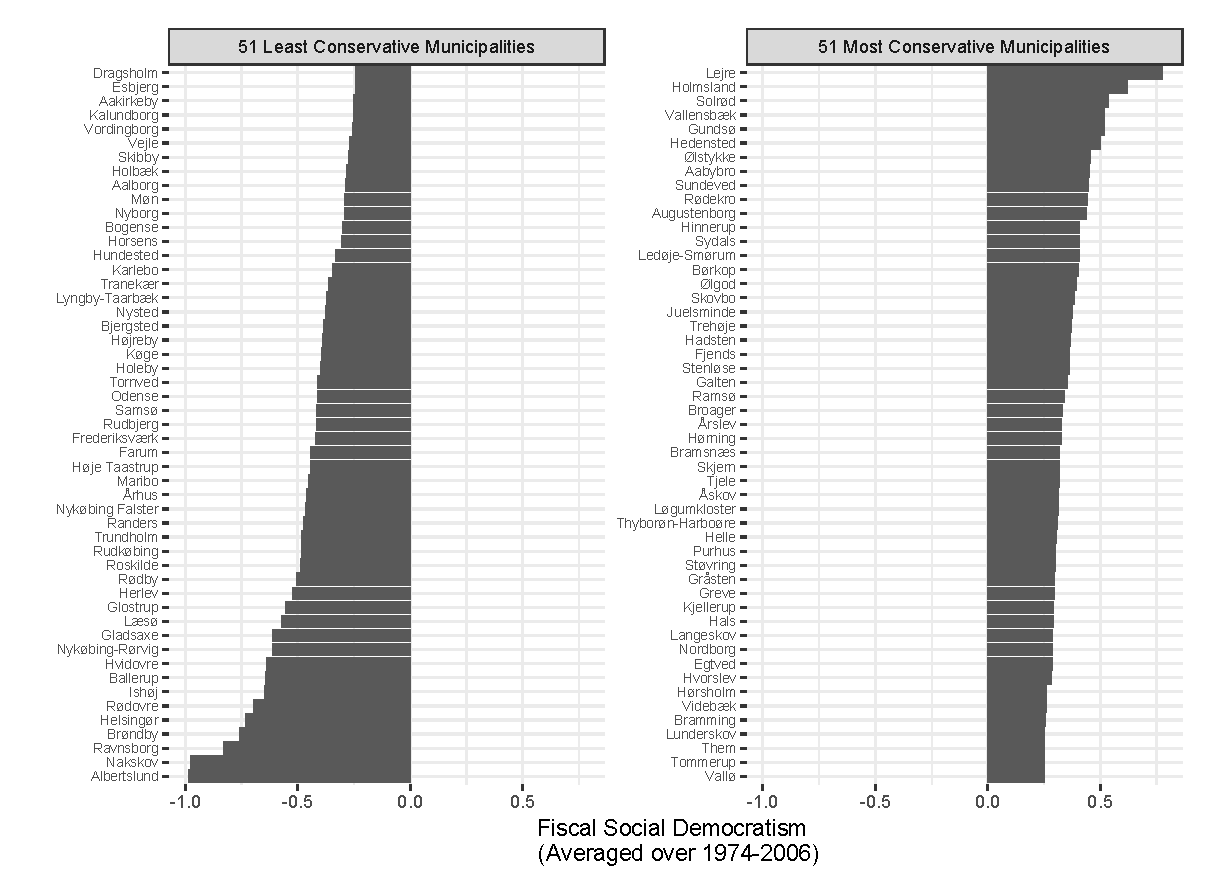
\includegraphics[width=1\textwidth]{conservatism_24092018.eps}
	\caption{The Most and Least Conservative Municipalities} \label{mostleast}
\end{figure}

\clearpage


\subsection{Validating Our Measure of Citizens' Policy Preferences} \label{validation}

\setcounter{table}{0}
\setcounter{figure}{0}


To have an indication of how well our electoral measure capture voters underlying preferences, we look at the 2013 Danish Municipal Election Survey \cite{elklit2017kv13}. In this survey, more than 30 respondents (avg. 46) from each municipality were asked to place themselves on an 11-point ideology scale going from left to right. We calculate the municipality-specific mean of these responses and correlate these with the municipality-specific net support for conservative parties in the 2013 municipal election.  As can be seen from Figure \ref{validation1}, the two are strongly correlated, which suggests that we are in fact tapping into relevant variation in policy views, when we measure citizens' preferences over parties. Further, it is important to note that the correlation is biased downwards, because we have random measurement error in our sample-based measure of policy views. The reader should also note that because of the municipal reform of 2006 (see section \ref{context})  we only have 98 observations corresponding to the 98 (amalgamated) municipalities.




\begin{figure}[htbp]
	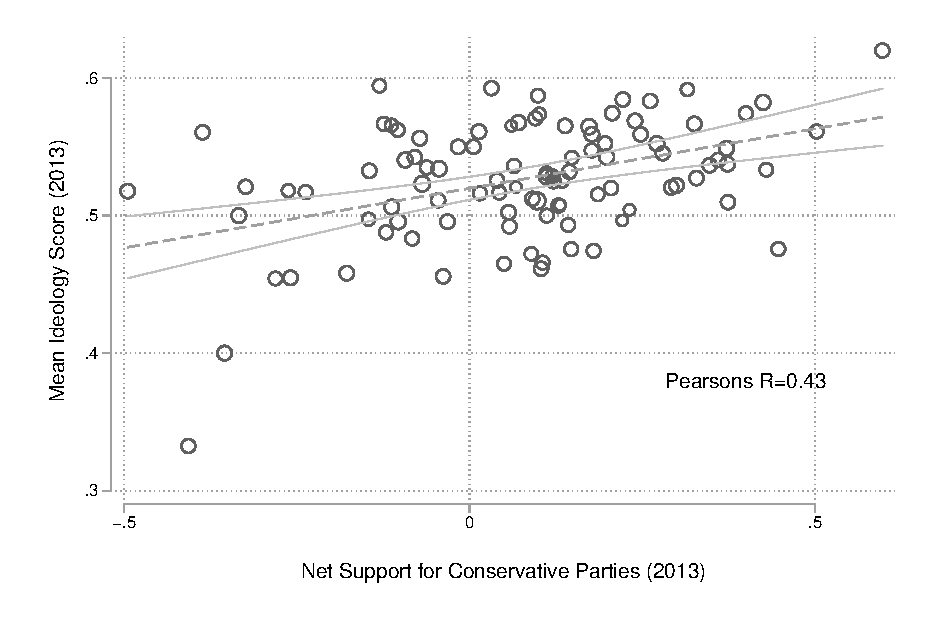
\includegraphics[width=1\textwidth]{validation1.eps}
	\caption{Does the electorates preference over parties reflect preferences over policy? Data from the 2013 municipal election.} \label{validation1}
\end{figure}  
\clearpage


\subsection{Are Changing Socio-demographics Driving Our Results?}\label{balance}

\setcounter{table}{0}
\setcounter{figure}{0}

In Table \ref{tab:balance}, we show how the electoral support for right-wing parties relates to changes in municipal socio-demographics. None of the correlations are strong. Unsurprisingly, given these low correlations, the coefficients are statistically indistinguishable from zero. Besides this, it should be noted that the model's overall explanatory power is very low, as indicated by the negative adjusted $R^2$.

\begin{table}[!htbp] \centering 
	\caption{Support for Right-Wing Parties and Socio Demographics.} 
	\label{tab:balance} 
	\begin{tabular}{@{\extracolsep{5pt}}lc} 
		\\[-1.8ex]\hline 
		\hline \\[-1.8ex] 
		& \multicolumn{1}{c}{\textit{Dependent variable:}} \\ 
		\cline{2-2} 
		\\[-1.8ex] & Electoral Support for Right-Wing Parties \\ 
		\hline \\[-1.8ex] 
		Education & $-$0.007 \\ 
		& (0.005) \\ 
		& \\ 
		Immigrants & $-$0.0001 \\ 
		& (0.0001) \\ 
		& \\ 
		Unemployed & $-$0.003 \\ 
		& (0.002) \\ 
		& \\ 
		\hline \\[-1.8ex] 
		Wald Stat & 2.22 \\ 
		Municipality? & Yes \\ 
		Year FE? & Yes \\ 
		Observations & 818 \\ 
		Adjusted R$^{2}$ & $-$0.500 \\ 
		\hline 
		\hline \\[-1.8ex] 
		\multicolumn{2}{p{10 cm}}{\emph{Note: Robust standard errors clustered on municipality are in parentheses. P value for the wald statistic is 0.53.}}\\ 
	\end{tabular} 
\end{table} 
\clearpage

\subsection{Does Fiscal Policy Affect Voter Preferences?}\label{granger}

\setcounter{table}{0}
\setcounter{figure}{0}

As an additional test of reverse causality, we use the lag of municipal policy as the explanatory variable in a series of fixed effects models predicting electoral support for right-wing parties. We use one- through four-year lags and report the result of each of these models in  \ref{fig:granger}. All coefficients are small and statistically insignificant. This strengthens our claim that changes in voter preferences leads to changes in policy and not the other way around.


\begin{figure}[!htb]
	\centering
	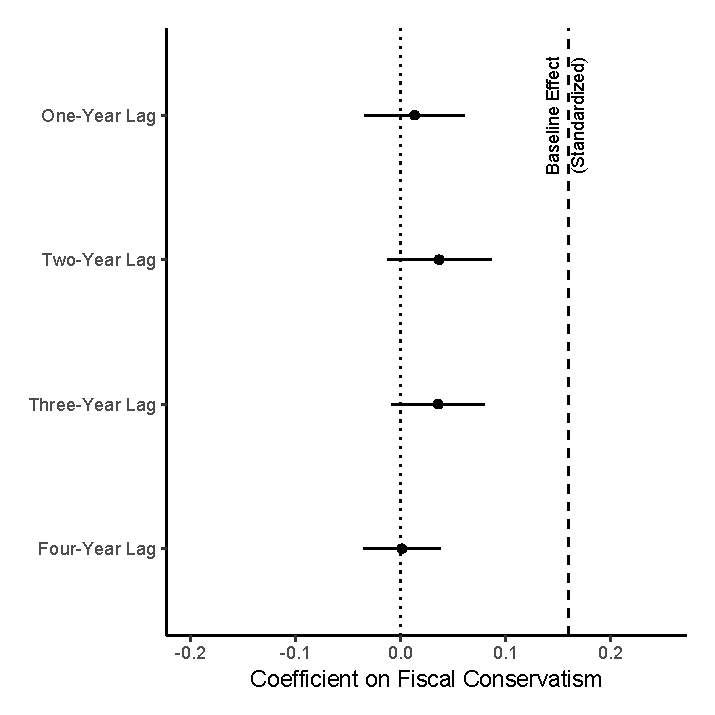
\includegraphics[scale = 1]{granger_18092018.eps}
	\caption{Reverse Causality? Fiscal Conservatism does not predict future support for Right-Wing parties. Confidence intervals are 95 percent, computed using robust standard errors clustered at the municipality level.} \label{fig:granger}
\end{figure}
\clearpage
\subsection{Is It Just the Mayoralty?}\label{mechanism}

There are two important reasons why we would expect municipal policy to be responsive to voter preferences. First, when the electorate chooses to elect more right-wing candidates, we would expect them to enact more fiscally conservative policies. Second, we might observe that parties are differentially responsive to voter preferences. We investigate these mechanisms in Figure \ref{fig:mech}.

In panel A, we include a categorical control for whether the mayoral party is the Liberal Party, the Social Democrats, or some third party.  In doing so, we condition the effect of electoral support for right-wing parties on whether those parties control the most important municipal policy-making position. This gives us the effect of support for right-wing parties among the voters after taking into account, which politicians they elect. Identifying the direct effect of electoral support net of selection by including a post-treatment control in this way requires very strong assumptions that are unlikely to be met. Still, it is striking how little the coefficient on policy preferences change, when we control for which party controls the mayoralty. 

\begin{figure}[!htb]
	\begin{subfigure}{0.45\textwidth}
		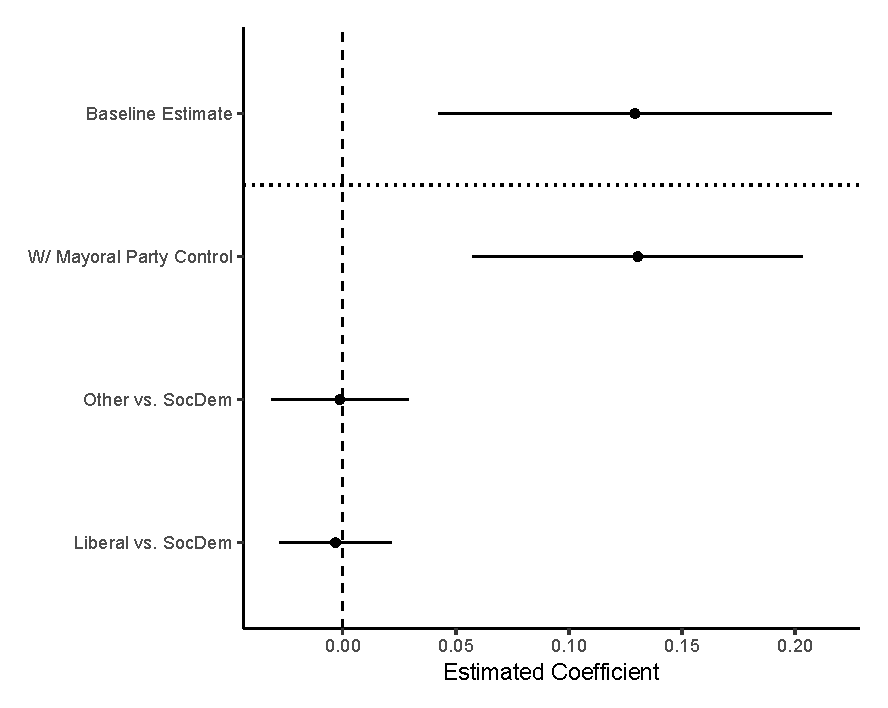
\includegraphics[width=1\textwidth]{PostTreatControl.eps}
		\caption{Are Results Driven by Selection? The figure shows results after including control for the mayoral party. Baseline estimates are included for comparison.} \label{mech}
	\end{subfigure}  \hfill
	\begin{subfigure}{0.45\textwidth}
		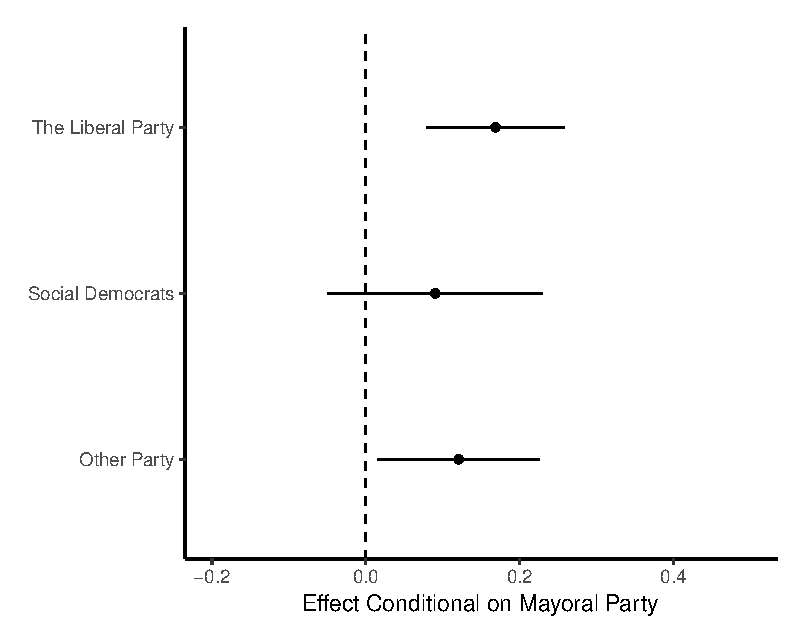
\includegraphics[width=1\textwidth]{MargFX_31082018.eps}
		\caption{Are All Parties Equally Responsive? The figure shows the marginal effects from a model including an interaction between mayoral party and electoral support for right-wing parties.} \label{inter}
	\end{subfigure}
	\caption{Responsiveness or Selection? Twoway fixed effects and population size (logged) included in both models. Confidence intervals are 95 pct., computed from robust standard errors with clustering at the municipal level.}
	\label{fig:mech}
\end{figure}

In panel B, we allow the effect to vary across our three different categories of mayoral party. The differences in the estimates are very small, suggesting that all mayors are equally responsive.

\clearpage

\subsection{Effects on Individual Policy Indicators}
\label{item}
\setcounter{table}{0}
\setcounter{figure}{0}


As our measure of municipal policy is made up of many different fiscal policies it is interesting to investigate, which factor(s) drive the effect. To do so, we regress a four-year lead of all policy items presented in Table \ref{tab:policies} individually on the electoral support of right-wing parties including time and year fixed effects. Figure \ref{fig:item} presents the results. While some variables are uncorrelated with voter preferences, a majority are quite strongly correlated with preferences, but the individual correlation is estimated with a great deal of uncertainty. This suggests that combining the items has added value over only using one, as we reduce statistical noise in the estimation process. 

\begin{figure}[!htb]
	\centering
	
\includegraphics[scale = 1]{ItemByItem_18092018.eps}
	\caption{Effect of Right-Wing Electoral Support Across Components of our Measure. Note that all measures of taxes and spending are reversed to capture that higher values equal more conservative policy. Confidence intervals are 95 percent, computed using robust standard errors clustered at the municipality level.} \label{fig:item}
\end{figure}
\clearpage



\subsection{Stability of Effects Across Time}
\label{stability}

\begin{figure}[!htb]
	\centering
	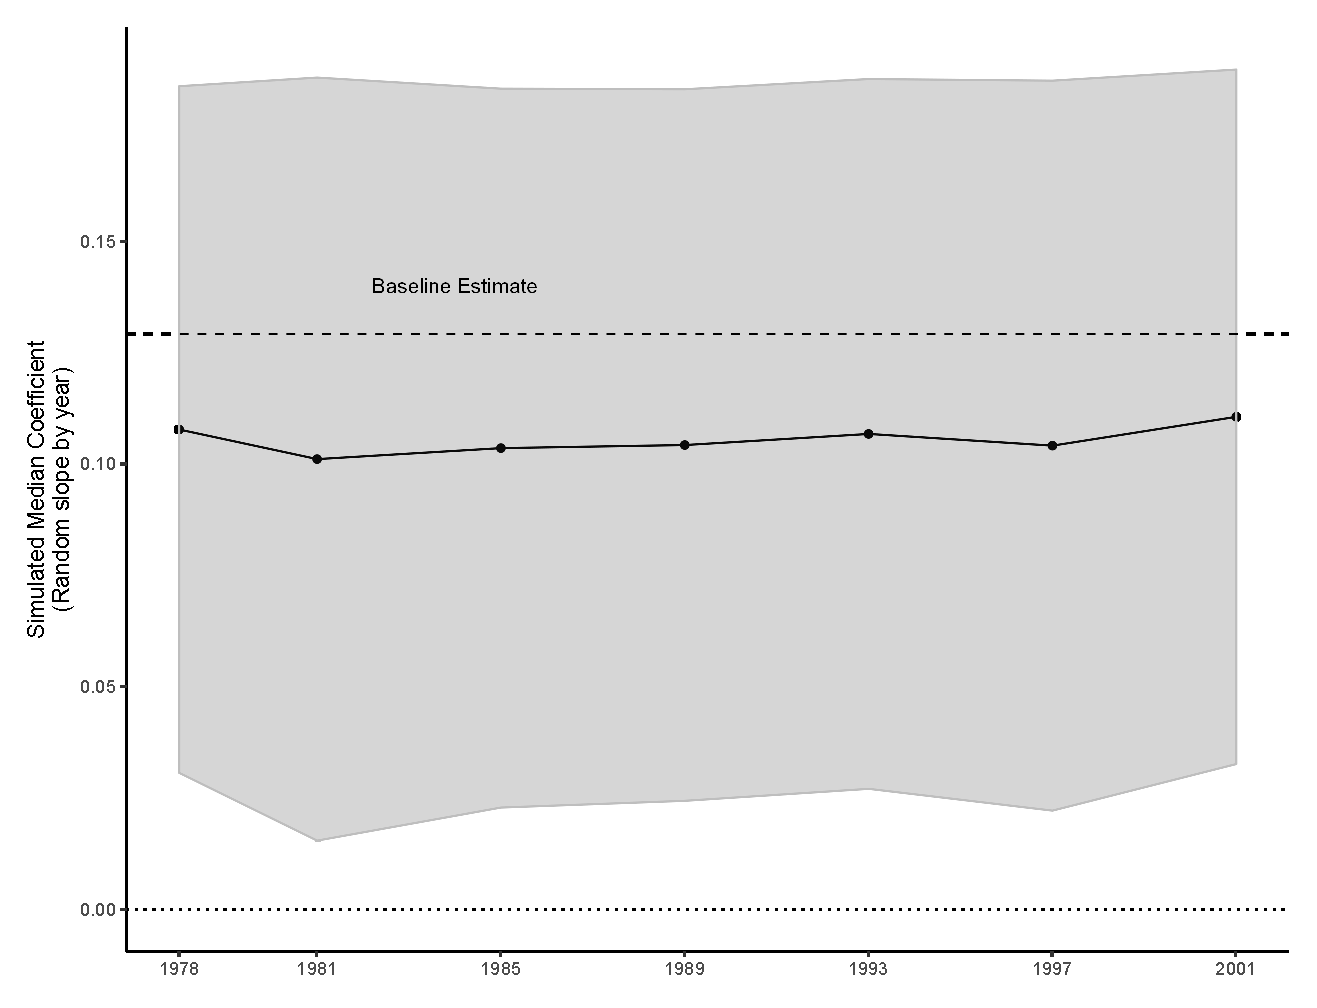
\includegraphics[scale = .65]{StabilityOfEffects.eps}
	\caption{How Stablea Feature is Dynamic Responsiveness? Points are estimates of random slopes by year with a lagged dependent variable to deal with autocorrelation. Shaded area is a 95 percent CI from the relevant percentiles of a bootstrapped distribution from 100 resamples.} \label{fig:stab}
\end{figure}

\bibliographystyle{apa}
\bibliography{library}


\end{document}